\documentclass[10pt,aspectratio=169]{beamer}

\usepackage{../../common/foundationsmacro-beamer}
\usepackage[english]{babel}
\usepackage{amsmath}
\usepackage{amssymb}
\usepackage{graphicx}
\usepackage{booktabs}
\usepackage{tikz}

% -----------------------------------------------------------------------------
% -- Title page and outline options ---- --------------------------------------
% -----------------------------------------------------------------------------

\title{Chapter II: A Model of Production}

\author[Bueren]{Jes\'{u}s Bueren}

\institute[Cat\'{o}lica-Lisbon ] % (optional, but mostly needed)
{

Cat\'{o}lica-Lisbon   

}

\date{}


%%%%%%%%%%%%%%%%%%%%%%%%%%%%%%%%%%%%%%%%%%%%%%%%%%%%%%




%%%%%%%%%%%%%%%%%%%%%%%%%%%%%%%%%%%%%%%%%%%%%%%%%%%%%%%%%%%%%%%%%%%%%%%%
\definecolor{darkgreen}{rgb}{0.0, 0.5, 0.0}
\definecolor{lightblue}{rgb}{0.3, 0.5, 0.55}
\definecolor{lightblue}{rgb}{0.3, 0.5, 0.55}
\definecolor{colormodel}{rgb}{0.3, 0.5, 0.55}



\begin{document}
\begin{frame}[plain]
    \titlepage
\end{frame}
\section{Introduction}


\begin{frame}{Two Ways to Answer Big Economic Questions}

\begin{itemize}

    \item There are two main approaches in economics:

    \vspace{0.2cm}

    \item \textbf{1. Empirical approach}
    \begin{itemize}
        \itemvso Use data to estimate causal effects.
        \itemvso Look for natural experiments.
        \itemvso Compare treated vs. control groups.
    \end{itemize}

    \vspace{0.3cm}

    \item \textbf{2. Theoretical approach}
    \begin{itemize}
        \itemvso Build a model of the whole economy.
        \itemvso Make assumptions explicit.
        \itemvso Study how all markets adjust simultaneously.
    \end{itemize}
    \itemvso If possible, combining both approaches is the best way to answer questions in economics.
\end{itemize}

\end{frame}

\begin{frame}{Why Isn't Empirical Evidence Enough?}

\begin{itemize}

    \item First problem: \textbf{No natural experiment for everything}

    \begin{itemize}
        \itemvso We cannot randomly assign an economy to “AI revolution”.
    \end{itemize}

    \itemvso Second problem: equilibrium effects

    \begin{itemize}
        \itemvso A policy affects one group...
        \itemvso But prices adjust for everyone
        \itemvso Other markets respond.
        \itemvso No control group
    \end{itemize}

\itemvso To understand how prices and quantities adjust, we need a model.
\end{itemize}

\end{frame}


\begin{frame}{An Economic Model Is Like a Video Game}
\begin{itemize}
    \item A model is just a mathematical representation of a hypothetical world.
    \itemvso Imagine designing a simple video game:
    \begin{itemize}
        \item You create a world and give it resources.
        \item You specify what the characters can do and how they make decisions.
        \item You work out what happens when they interact.
    \end{itemize}

    \itemvso Building an economic model follows the same logic:
    \begin{itemize}
        \item Specify the available workers, machines, and technology.
        \item Describe how households and firms make decisions.
        \item Find the resulting output, wages, and rental rates.
    \end{itemize}

    \itemvso We can then use the video game to answer questions about the world we created.
    \itemvso In this chapter, we will build a simple model of production and use it to understand why some countries are rich and others are poor.
\end{itemize}
\end{frame}


\section{A Production Function}
\begin{frame}{Production Function}

\begin{itemize}
    \item First step: describe how the economy produces output.
    \itemvso Economists summarize this with a production function:
    \[
    Y = F(K, L)
    \]
    \vspace{-0.3cm}
    \item Output depends on:
    \begin{itemize}
        \item $L$ — workers (labor)
        \item $K$ — machines
    \end{itemize}

    \itemvso This simple relationship will not only determine output determine wages and profits.
\end{itemize}

\end{frame}


\begin{frame}{What Happens When We Add More Workers?}

\begin{itemize}
    \item Hold capital fixed ($K$ constant).
    \itemvso Suppose the labor force increases (migration) or decreases (aging).
    \itemvso We assume that adding more workers has two effects:
    \begin{itemize}
        \item Total output rises — more hands help produce more. 
        \item But each additional worker adds a bit less than the previous one — they share the same capital and tools.
    \end{itemize}


    \itemvso Mathematically, we capture this with:
    \begin{itemize}
        \itemvso Positive marginal product: $\frac{\partial F}{\partial L} > 0$
        \itemvso Diminishing marginal product: $\frac{\partial^2 F}{\partial L^2} < 0$
    \end{itemize}
\end{itemize}

\end{frame}

\begin{frame}{What Happens When We Add More Machines?}

\begin{itemize}
    \item Hold labor fixed ($L$ constant).
    \itemvso Suppose the firm invests in more machines or equipment.

    \itemvso We assume that adding more capital has two effects:
    \begin{itemize}
        \itemvso Total output rises — more machines help produce more. 
        \itemvso But each additional machine adds a bit less than the previous one — workers have only so much to operate.
    \end{itemize}


    \itemvso Mathematically, we capture this with:
    \begin{itemize}
        \itemvso Positive marginal product: $\frac{\partial F}{\partial K} > 0$
        \itemvso Diminishing marginal product: $\frac{\partial^2 F}{\partial K^2} < 0$
    \end{itemize}

    \vspace{0.3cm}

\end{itemize}

\end{frame}


\begin{frame}{Cobb--Douglas Production Function}

\begin{itemize}
    \item A very popular production function in macro is the Cobb--Douglas:
    \[
        Y = A K^{\alpha} L^{1-\alpha}
    \]
    \vspace{-0.4em}
    \item $A$ measures productivity: how good the economy is at turning inputs into output.
    \itemvso The marginal products are easy to compute:
    \[
        \frac{\partial Y}{\partial L}
        = (1-\alpha) A K^{\alpha} L^{-\alpha} \ge 0,
        \qquad
        \frac{\partial Y}{\partial K}
        = \alpha A K^{\alpha-1} L^{1-\alpha} \ge 0
    \]
    \vspace{-0.4em}
    \item And both marginal products get smaller as we increase that input:
    \[
        \frac{\partial^2 Y}{\partial L^2} \le 0, \qquad
        \frac{\partial^2 Y}{\partial K^2} \le 0
    \]
    \vspace{-0.4em}
    \item The two inputs also help each other:
    \[
        \frac{\partial^2 Y}{\partial K \partial L} = \alpha(1-\alpha)A K^{\alpha-1} L^{-\alpha} \ge 0
    \]
    Adding machinery raises how much extra output you get from hiring an extra worker
\end{itemize}

\end{frame}

\begin{frame}{Returns to Scale: What Happens if We Grow Everything?}

\begin{itemize}
    \item Recall our Cobb--Douglas technology:
    \[
        Y = A K^{\alpha} L^{1-\alpha}
    \]
    \vspace{-0.3cm}
    \item What happens if we double both capital and labor? 
    \[
        F(2K, 2L) = A (2K)^\alpha (2L)^{1-\alpha} = 2 \, F(K,L)
    \]
    \vspace{-0.3cm}
    \item Doubling inputs gives exactly double output — this is called \textbf{constant returns to scale}.
\end{itemize}

\end{frame}

\begin{frame}{Why Constant Returns to Scale?}

\begin{itemize}
    \item For Cobb--Douglas, returns to scale depend on the sum of the exponents:
    \[
        \alpha + (1-\alpha) = 1
    \]
    \itemvso If the sum is:
    \begin{itemize}
        \item Equal to 1: constant returns to scale
        \item Greater than 1: increasing returns 
        \item Less than 1: decreasing returns
    \end{itemize}
\end{itemize}

\end{frame}

\section{Firm's problem}

\begin{frame}{Firm's Problem}

\begin{itemize}
    \item Second step: describe how firms choose labor and capital.
    \itemvso So far, we have seen how output responds to changes in labor and capital.
    \itemvso Firms choose $K$ and $L$ to maximize profits:
    \[
        \max_{K,L} \ F(K,L) - r K - w L
    \]
    \vspace{-0.4em}
    \item Profits = production minus cost of inputs.
    \itemvso We set the price of output to 1 (numeraire).
    \itemvso $r$ = rental price of capital, $w$ = wage of workers.
    \itemvso Firms take $r$ and $w$ as given because markets are competitive 
    (simplifying assumption — left-wing critique possible).
\end{itemize}

\end{frame}


\begin{frame}{Firm's Problem: Solution}

\begin{itemize}
    \item Profit-maximization problem:
    \[
        \max_{K,L} \Pi(K,L)=\max_{K,L}  \ F(K,L) - r K - w L
    \]
    \vspace{-0.2cm}
    \item[-] Step 1: Choose optimal capital \(K\)  (hold \(L\) fixed)
    \item[-] Step 2: Choose optimal labor \(L\)  (hold \(K\) fixed)
    \itemvso We will see that the solution satisfies:
    \[
        \text{MP}_K(K^*,L^*)=\dfrac{\partial F(K^*,L^*)}{\partial K} = r, \quad \text{MP}_L(K^*,L^*)=\dfrac{\partial F(K^*,L^*)}{\partial L}  = w
    \]
    Just like in micro: hire/rent until marginal revenue = marginal cost.
    \itemvso $\text{MP}_K$ and $\text{MP}_L$ are the marginal product of capital and labor.
\end{itemize}

\end{frame}

\begin{frame}{Maximization in Two Variables}

\begin{itemize}
    \item General math rule:
    \[
        \max_{x,y} f(x,y)
    \]
    \vspace{-0.2cm}
    \item Solution satisfies first-order conditions:
    \[
        \frac{\partial f(x^*,y^*)}{\partial x} = 0, \quad \frac{\partial f(x^*,y^*)}{\partial y} = 0
    \]
    \vspace{-0.2cm}
    \item Applied to the firm:
    \[
        \frac{\partial \Pi(K^*,L^*)}{\partial K} = 0, \quad \frac{\partial \Pi(K^*,L^*)}{\partial L} = 0
    \]
    \item Hire each input until marginal revenue of the input = cost of the input (just like MR = MC in micro for one good).
\end{itemize}

\end{frame}

\begin{frame}{Firm's Problem with Cobb--Douglas}

\begin{itemize}
    \item Profit function:
    \[
        \Pi(K,L) = F(K,L) - rK - wL
    \]
    \item Cobb--Douglas:
    \[
        \Pi(K,L) = A K^\alpha L^{1-\alpha} - rK - wL
    \]
    \itemvso Goal: choose \(K\) and \(L\) to maximize profits.
    \itemvso Taking the derivative and equating to zero we get:
    \[
        \alpha A K^{\alpha-1} L^{1-\alpha} -r =0 , \quad 
        (1-\alpha) A K^\alpha L^{-\alpha} - w=0 
    \]
    \[
       \text{MP}_K= \alpha A K^{\alpha-1} L^{1-\alpha} =r , \quad 
        \text{MP}_L=(1-\alpha) A K^\alpha L^{-\alpha} = w 
    \]
    \item Hire inputs until MP = price (marginal revenue = marginal cost).
\end{itemize}

\end{frame}

\begin{frame}{Firm's Problem}{Example: Hiring Labor with Fixed Capital}

\begin{itemize}
    \item Imagine that you own 1 machine and decide how many workers to hire.
    \itemvso Profit function:
    \[
        \Pi(K,L) = A K^\alpha L^{1-\alpha} - w L
    \]
    \vspace{-0.3cm}
    \item FOC for labor:
    \[
        \frac{\partial \Pi}{\partial L} = A(1-\alpha) K^\alpha L^{-\alpha} - w = 0
    \]
    \vspace{-0.3cm}
 \item Numbers: \(A=1, \alpha=0.5, K=1, w=0.25\)
    \[
        0.5 \cdot 1^{0.5} L^{-0.5} - 0.25 = 0 \implies L = 4
    \]
    \vspace{-0.3cm}
    \item Hire workers until marginal product of labor = wage.
\end{itemize}

\end{frame}

\begin{frame}{Firm's Problem}{Example: Hiring Labor with Fixed Capital}

\begin{columns}[T]

% ===== LEFT COLUMN =====
\begin{column}{0.57\textwidth}

\begin{itemize}
    \item Marginal product of labor:
    \[ \text{MP}_L = (1-\alpha) A K^\alpha L^{-\alpha} \]
    \item Downward sloping: each additional worker adds less output.
    \itemvso Horizontal line = wage $w$.
    \itemvso Hire labor until:
    \[ \text{MP}_L = w \]
    \vspace{-0.5cm}
    \item Intersection shows optimal number of workers $L^*$.
    \item This curve is called the labor demand curve.
\end{itemize}

\end{column}

% ===== RIGHT COLUMN =====
\begin{column}{0.45\textwidth}

\begin{center}
% Show the relevant range around the hiring decision, away from L = 0.
\begin{tikzpicture}[x=0.65cm, y=6cm, every node/.style={font=\small}]

  % Parameters
  \def\A{1}    
  \def\capitalExponent{0.5}  
  \def\K{1}    
  \def\w{0.25} 
  \pgfmathsetmacro{\Lstar}{((1-\capitalExponent)*\A*\K^\capitalExponent/\w)^(1/\capitalExponent)}

  % Axes
  \draw[->, thick] (0,0) -- (6.5,0) node[right] {$L$};
  \draw[->, thick] (0,0) -- (0,0.5) node[above] {$\text{MP}_L, w$};

  % Exact Cobb--Douglas MPL, showing its gentler portion near L* = 4.
  \draw[ultra thick, MacroBlue, domain=2:6, samples=100, smooth]
    plot (\x,{(1-\capitalExponent)*\A*\K^\capitalExponent*\x^(-\capitalExponent)});
  \node[above] at (2.2,0.36) {$\text{MP}_L$};
  
  % Wage Line (Thicker)
  \draw[ultra thick, red] (0,\w) -- (6,\w);

  % Mark the hiring optimum and project it onto the labor axis.
  \draw[dashed, gray!80, thick] (\Lstar,0) -- (\Lstar,\w);
  \node[circle, fill=black, inner sep=1.7pt] at (\Lstar,\w) {};

  \node[left] at (0,\w) {$\color{red}w = 0.25$};

  % Keep the axis labels focused on the relevant range and the optimum.
  \foreach \x in {2,6}
      \draw (\x,0.008) -- (\x,-0.008) node[below, text=gray] {\x};
  \draw (\Lstar,0.008) -- (\Lstar,-0.008)
      node[below] {$L^* = 4$};

\end{tikzpicture}
\end{center}

\end{column}

\end{columns}

\end{frame}



\begin{frame}{Firm's Problem}{Example: Renting Capital with Fixed Labor}

\begin{itemize}
    \item Imagine that you employ 1 worker and decide how many machines to rent.
    \itemvso Profit function:
    \[
        \Pi(K,L) = A K^\alpha L^{1-\alpha} - r K
    \]
    \vspace{-0.3cm}
    \item FOC for capital:
    \[
        \frac{\partial \Pi}{\partial K} = \alpha A K^{\alpha-1} L^{1-\alpha} - r = 0
    \]
    \vspace{-0.3cm}
    \item Numbers: \(A=1, \alpha=0.5, L=1, r=0.25\)
    \[
        0.5 \cdot 1^{0.5} K^{-0.5} - 0.25 = 0 \implies K = 4
    \]
    \vspace{-0.3cm}
    \item Rent machines until marginal product of capital = rental price.
\end{itemize}

\end{frame}

\begin{frame}{Firm's Problem}{Example: Renting Capital with Fixed Labor}

\begin{columns}[T]

\begin{column}{0.57\textwidth}

\begin{itemize}
    \item Marginal product of capital:
    \[ \text{MP}_K = \alpha A K^{\alpha-1} L^{1-\alpha} \]
    \item Downward sloping: each additional machine adds less output.
    \itemvso Horizontal line = rental price $r$.
    \itemvso Rent capital until:
    \[ \text{MP}_K = r \]
    \vspace{-0.5cm}
    \item Intersection shows optimal number of machines $K^*$.
    \item This curve is called the capital demand curve.
\end{itemize}

\end{column}

\begin{column}{0.45\textwidth}

\begin{center}
% Match the labor example, showing the relevant range away from K = 0.
\begin{tikzpicture}[x=0.65cm, y=6cm, every node/.style={font=\small}]

  % Parameters
  \def\A{1}
  \def\capitalExponent{0.5}
  \def\L{1}
  \def\r{0.25}
  \pgfmathsetmacro{\Kstar}{(\capitalExponent*\A*\L^(1-\capitalExponent)/\r)^(1/(1-\capitalExponent))}

  % Axes
  \draw[->, thick] (0,0) -- (6.5,0) node[right] {$K$};
  \draw[->, thick] (0,0) -- (0,0.5) node[above] {$\text{MP}_K, r$};

  % Exact Cobb--Douglas MPK, showing its gentler portion near K* = 4.
  \draw[ultra thick, MacroBlue, domain=2:6, samples=100, smooth]
    plot (\x,{\capitalExponent*\A*\L^(1-\capitalExponent)*\x^(\capitalExponent-1)});
  \node[above] at (2.2,0.36) {$\text{MP}_K$};

  % Rental price
  \draw[ultra thick, red] (0,\r) -- (6,\r);

  % Mark the rental optimum and project it onto the capital axis.
  \draw[dashed, gray!80, thick] (\Kstar,0) -- (\Kstar,\r);
  \node[circle, fill=black, inner sep=1.7pt] at (\Kstar,\r) {};
  \node[left] at (0,\r) {$\color{red}r = 0.25$};

  \foreach \x in {2,6}
      \draw (\x,0.008) -- (\x,-0.008) node[below, text=gray] {\x};
  \draw (\Kstar,0.008) -- (\Kstar,-0.008)
      node[below] {$K^* = 4$};

\end{tikzpicture}
\end{center}

\end{column}

\end{columns}

\end{frame}

\begin{frame}{Capital and Labor Supply}

\begin{itemize}

\item We have seen how firms choose capital and labor to maximize profits

\itemvso Firms' decisions determine factor demand

\itemvso Now we introduce factor supply.

\itemvso Simplifying assumption:
\[
K^{s} = \overline{K}, 
\qquad 
L^{s} = \overline{L}
\]
(Fixed total amounts in the economy.)


\end{itemize}

\end{frame}

\section{Equilibrium}
\begin{frame}{Model Summary}

\begin{itemize}
\item Last step: find the equilibrium.
\itemvso In \textbf{general equilibrium}, prices and quantities adjust so that all markets clear simultaneously. Our model has five equations:

\itemvso Capital demand: \quad $\alpha A K^{\alpha-1} L^{1-\alpha} = r$

\itemvso Labor demand: \quad $(1-\alpha) A K^{\alpha} L^{-\alpha} = w$

\itemvso Capital supply: \quad $K = \overline{K}$

\itemvso Labor supply: \quad $L = \overline{L}$

\itemvso Production function: \quad $Y = A K^{\alpha} L^{1-\alpha}$

\itemvso The five endogenous variables are: $K$, $L$, $r$, $w$, and $Y$.

\end{itemize}

\end{frame}


\begin{frame}{An Equilibrium}

\begin{itemize}

\item In economics, the solution to a model is called an equilibrium. 

\itemvso Equilibrium describes what happens when all markets clear, that is, supply equals demand in each market. 

\itemvso In our model, we have five equations with five unknowns. 

\itemvso Solving the model means finding the values of the endogenous variables ($K$, $L$, $r$, $w$, $Y$) in terms of the exogenous variables ($\overline{K}$, $\overline{L}$, $A$, $\alpha$). 

\itemvso This involves rewriting the system so that all endogenous variables are on one side of the equations and only parameters and exogenous variables on the other side.

\end{itemize}

\end{frame}

\begin{frame}{Equilibrium Values}

\begin{itemize}

\item In our simple model, the equilibrium values are:

\itemvso Capital: $K = \overline{K}$

\itemvso Labor: $L = \overline{L}$

\itemvso Rental rate of capital: $r = \alpha A \overline{K}^{\alpha-1} \overline{L}^{1-\alpha}$

\itemvso Wage: $w = (1-\alpha) A \overline{K}^\alpha \overline{L}^{-\alpha}$

\itemvso Output: $Y = A \overline{K}^\alpha \overline{L}^{1-\alpha}$

\itemvso These values satisfy all five equations of the model and clear labor, capital and goods markets.

\end{itemize}

\end{frame}


\section{Why poor countries are poor?}
\begin{frame}{Development Accounting}
\begin{itemize}
\item We now make an important leap: we apply the production function of our model
to aggregate economies across the world.
\itemvso We match output per person in the model ($y$) to GDP per capita in the data.
\itemvso Capital ($k$) is measured as the economy's stock of housing, factories,
machines, and equipment, divided by population.
\itemvso The production function implies:
\[
y = A k^{1/3}.
\]
\vspace{-0.3cm}
\item For now, we make a strong simplifying assumption:
\begin{itemize}
    \itemvso Technology is the same across countries: \(A\) is constant across countries.
\end{itemize}
so that income differences depend \emph{only} on capital per person.
\end{itemize}
\end{frame}


\begin{frame}{US as a benchmark}

\begin{itemize}
    \item We use the \textbf{United States as a benchmark} to compare countries.

    \itemvso Measure each country's capital and output per person
    \textbf{relative to their US values}.

    \itemvso With equal productivity across countries, the model implies:
    \[
        \frac{y_i}{y_{\mathrm{US}}}
        = \frac{A k_i^{1/3}}{A k_{\mathrm{US}}^{1/3}}
        = \left(\frac{k_i}{k_{\mathrm{US}}}\right)^{1/3}.
    \]

    \itemvso A relative value of 1 means the same as the US;
    a value of 0.5 means half the US level.

    \itemvso The US is therefore located at \(\mathbf{(1,1)}\) on the graph.
\end{itemize}

\end{frame}

\begin{frame}{The Model Relative to the US}

\centering
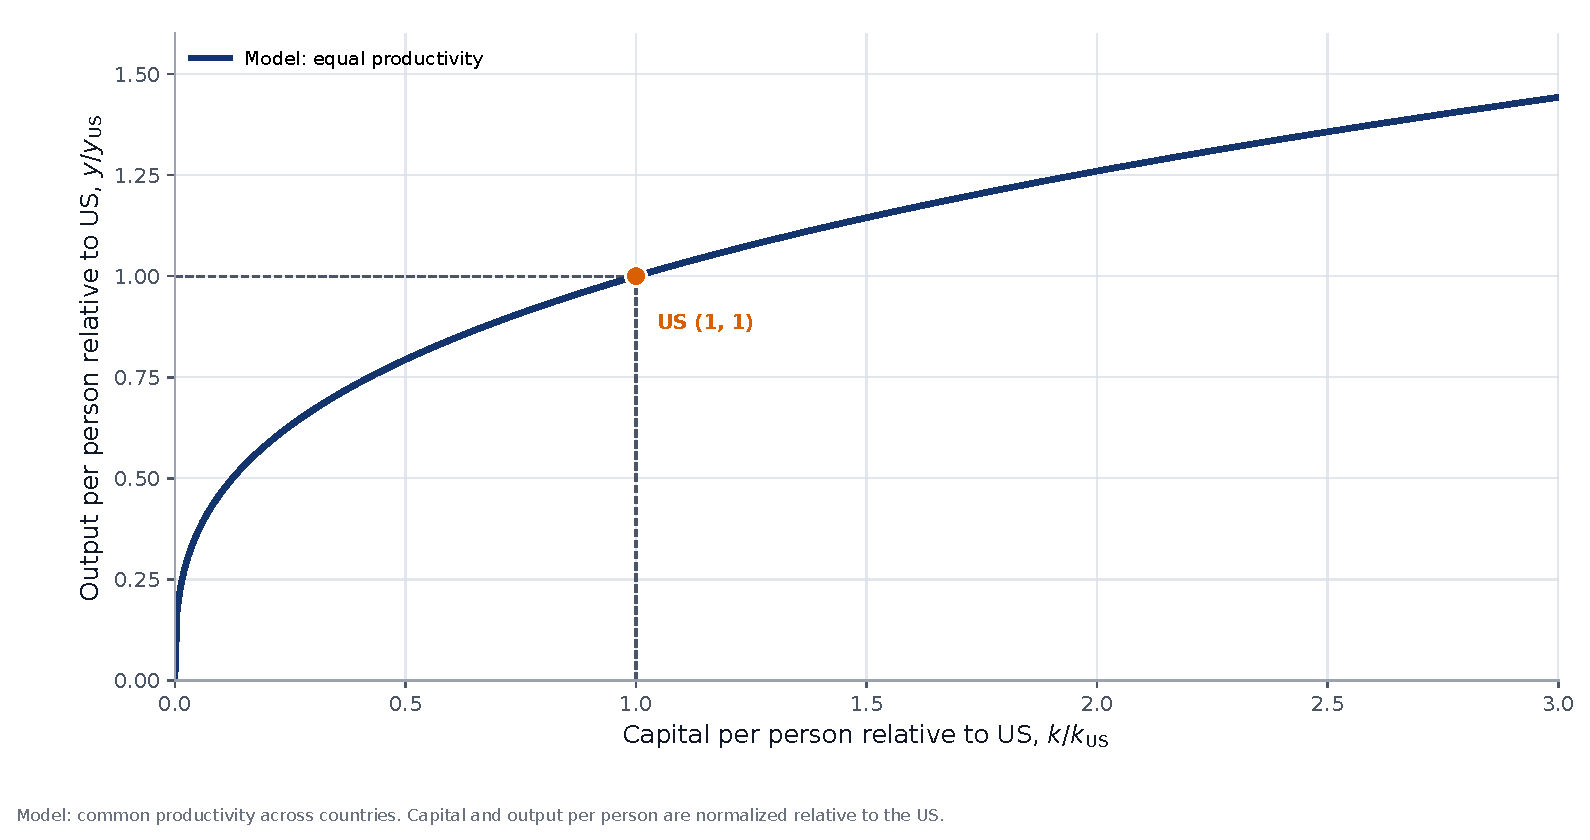
\includegraphics[width=0.96\linewidth,height=0.78\textheight,keepaspectratio]
{figures/Production_Model_Scatter_Relative_US_US_Only.pdf}

\end{frame}

\begin{frame}{Why Is the Curve Increasing and Concave?}

\begin{itemize}
    \item The curve shows the model's prediction when productivity is held fixed:
    \[
        \frac{y_i}{y_{\mathrm{US}}}
        = \left(\frac{k_i}{k_{\mathrm{US}}}\right)^{1/3}.
    \]

    \itemvso \textbf{Increasing:} more capital per person allows more output per person.

    \itemvso \textbf{Concave:} each additional unit of capital per person
    adds less output than the previous one.

    \itemvso Changing capital per person gives:
    \[
        \begin{aligned}
            \text{Doubling:}\quad &2^{1/3} \approx 1.26
            &&\text{(about 26\% more output per person)},\\[0.3em]
            \text{Halving:}\quad &(1/2)^{1/3} \approx 0.79
            &&\text{(about 21\% less output per person)}.
        \end{aligned}
    \]

    \item This is \textbf{diminishing returns to capital}.
\end{itemize}

\end{frame}

\begin{frame}{Predictions of the Model}

Consider Portugal as an example.

\medskip

\begin{itemize}
\item Capital per person in Portugal and Spain is close to or even slightly above
the U.S. level.
\end{itemize}

\medskip

According to the model:
\[
y = k^{1/3},
\]
so if $k_{\text{PRT}} \approx k_{\text{US}}$, the model predicts:
\[
y_{\text{PRT}} \approx y_{\text{US}} .
\]

 Therefore, according to the model, Portugal should be about as rich as the United States.

\medskip
\end{frame}

\begin{frame}{Production Model: Model vs Data}
\centering
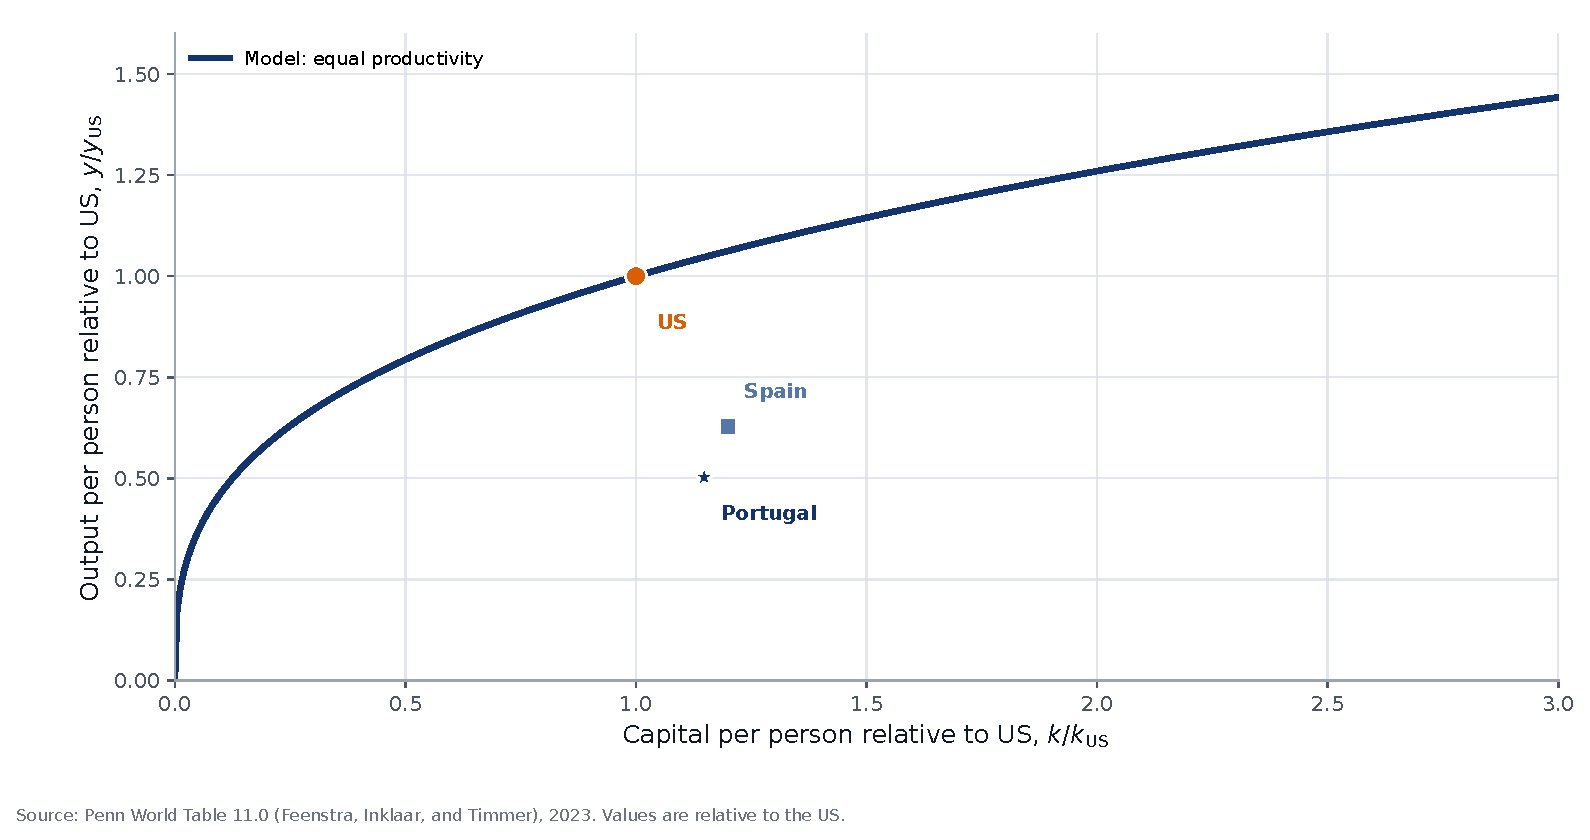
\includegraphics[width=0.96\linewidth,height=0.78\textheight,keepaspectratio]
{figures/Solow_K_Y_Curve_Relative_US.pdf}
\end{frame}

\begin{frame}{Production Model: Model vs Data}
\centering
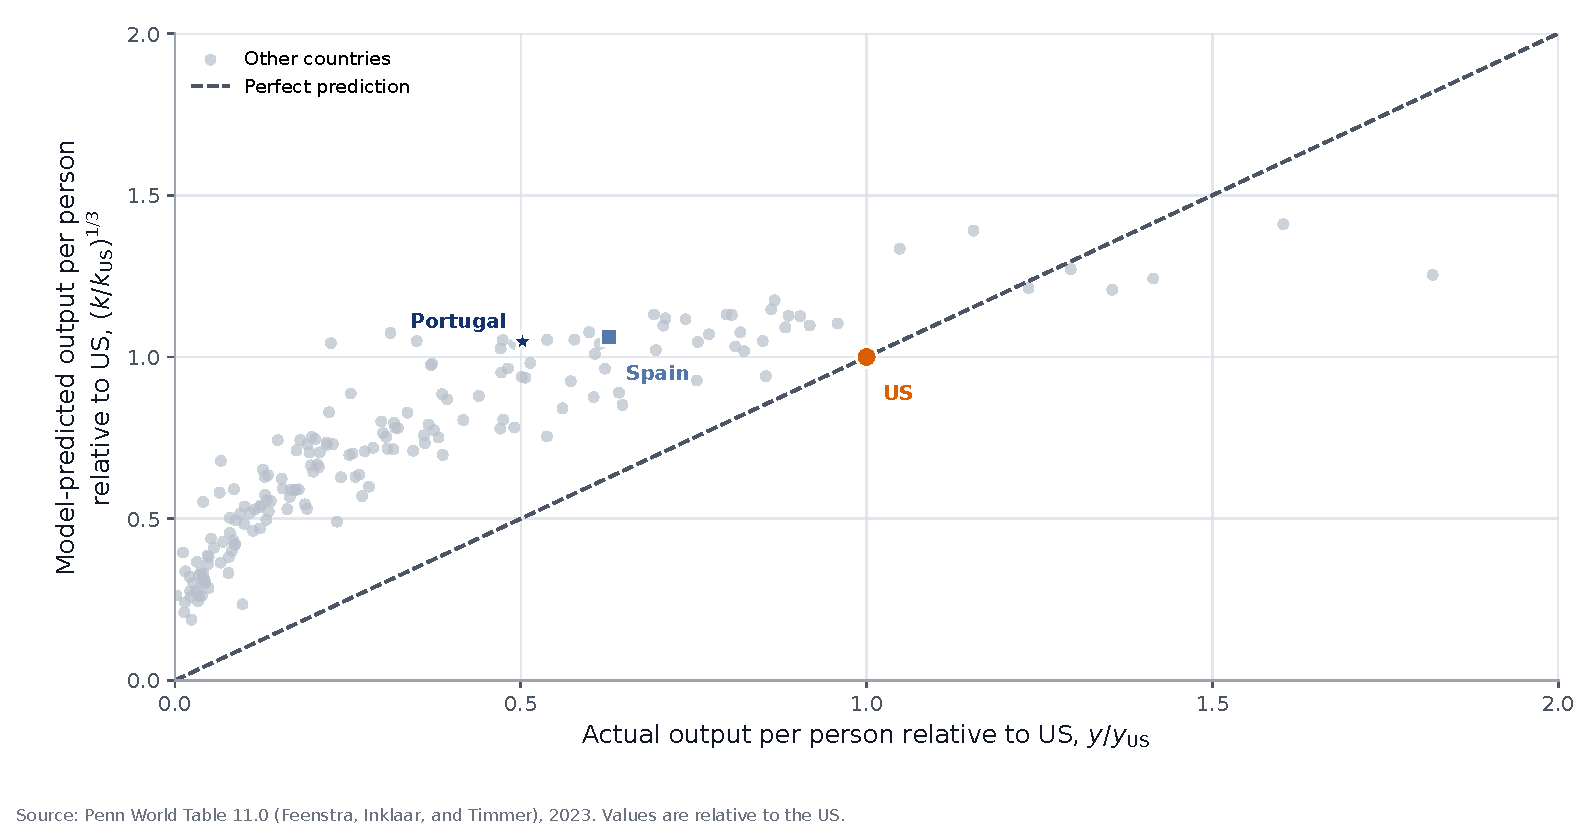
\includegraphics[width=0.96\linewidth,height=0.78\textheight,keepaspectratio]
{figures/Production_Model_Scatter_Relative_US.pdf}
\end{frame}


\begin{frame}{Model vs Data}
\begin{itemize}
\item In general, the model correctly predicts that countries are rich or poor
according to how much capital per person they have.
\itemvso However, the magnitudes are very wrong: the model underestimates how poor countries are relative to the U.S.
\itemvso One way to reconcile the model with the data is to allow the productivity
parameter $A$ to be country-specific.
\itemvso $A$ measures how productive countries are at using their factor inputs
(in this case, $K$ and $L$) to produce output.
\itemvso Thought experiment: what value of $A_{\text{PRT}}$ would rationalize why Portugal
produces much less output per capita than the U.S.?
\itemvso The inferred value of $A$ is referred to as total factor productivity (TFP).
\end{itemize}
\end{frame}

\begin{frame}{Production Model with Country-Specific TFP}
\centering
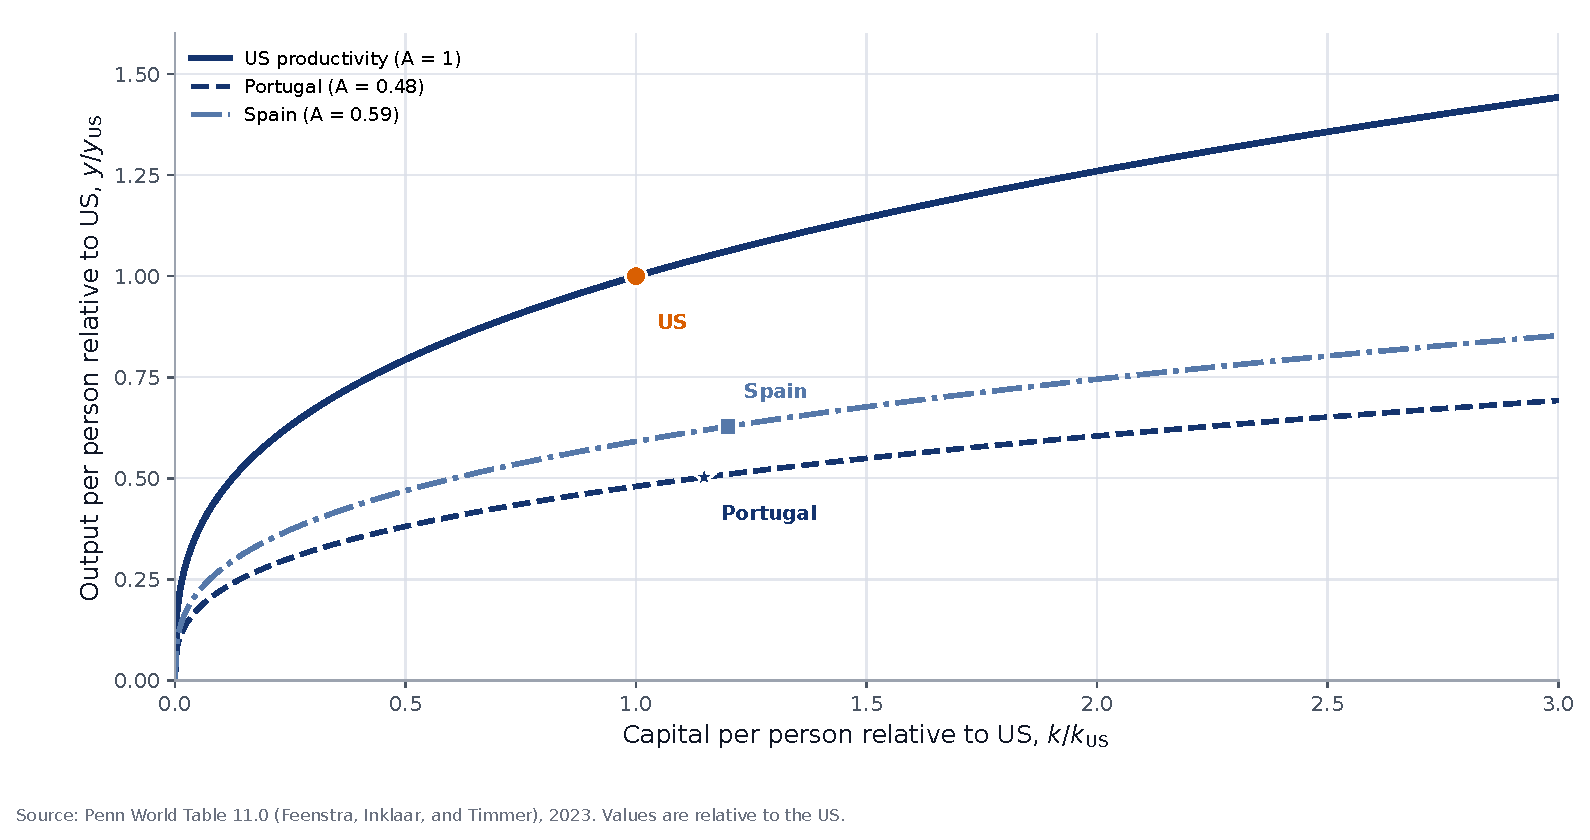
\includegraphics[width=0.96\linewidth,height=0.78\textheight,keepaspectratio]
{figures/Solow_K_Y_Curve_Country_TFP.pdf}
\end{frame}

\begin{frame}{Poor vs Rich Countries}
\begin{itemize}
    \item Rich countries have about \textbf{125 times as much capital per person}
    as poor countries:
    \[
        \frac{k_{\text{rich}}}{k_{\text{poor}}} \simeq 125.
    \]

    \itemvso With equal productivity, this would predict only a
    \textbf{5-fold gap in output per person}: \(125^{1/3}=5\).

    \itemvso In the data, output per person is about \textbf{70 times higher}
    in rich countries.
\end{itemize}

\[
    \underbrace{\frac{y_{\text{rich}}}{y_{\text{poor}}}}_{\simeq\,70}
    =
    \underbrace{\frac{A_{\text{rich}}}{A_{\text{poor}}}}_{\simeq\,14}
    \times
    \underbrace{\left(\frac{k_{\text{rich}}}{k_{\text{poor}}}\right)^{1/3}}_{\simeq\,5}.
\]

\begin{itemize}
    \itemvso The remaining gap is captured by \textbf{TFP} in the model:
    \(A_{\text{rich}}/A_{\text{poor}} \simeq 70/5 = 14\).
\end{itemize}
\end{frame}

\begin{frame}{Example: Cabo Verde}

\begin{itemize}
\item The US has about \textbf{5 times as much capital per person} as Cabo Verde:
\[
\frac{k_{\text{US}}}{k_{\text{CPV}}} \simeq 5.
\]
\itemvso With equal productivity, \(A_{\text{US}}=A_{\text{CPV}}\), the model predicts:
\[
\frac{y_{\text{US}}}{y_{\text{CPV}}}
= \frac{A_{\text{US}}}{A_{\text{CPV}}}
  \left(\frac{k_{\text{US}}}{k_{\text{CPV}}}\right)^{1/3}
= 5^{1/3} \approx 1.71.
\]

\itemvso In the data, the US has about \textbf{6.7 times as much output per person}:
\[
\frac{y_{\text{US}}}{y_{\text{CPV}}} \simeq \frac{1}{0.15} \approx 6.7.
\]

\itemvso Capital differences alone \textbf{underpredict the observed output gap}.

\end{itemize}

\end{frame}

\begin{frame}{Example: Cabo Verde}

\begin{itemize}

\item We infer \textbf{relative TFP} from the output and capital ratios:
\[
\frac{A_{\text{US}}}{A_{\text{CPV}}}
= \frac{y_{\text{US}}/y_{\text{CPV}}}
       {\left(k_{\text{US}}/k_{\text{CPV}}\right)^{1/3}}
\approx \frac{6.67}{1.71} \approx 3.9.
\]

\item Decomposing the income gap:
\[
\underbrace{\frac{y_{\text{US}}}{y_{\text{CPV}}}}_{\simeq\,6.7}
= \underbrace{\frac{A_{\text{US}}}{A_{\text{CPV}}}}_{\simeq\,3.9\ \text{(TFP)}}
\times \underbrace{\left(\frac{k_{\text{US}}}{k_{\text{CPV}}}\right)^{1/3}}_{\simeq\,1.7\ \text{(capital)}}.
\]
\itemvso If Cabo Verde had US productivity, its output per person would be about
\textbf{3.9 times higher}.
\itemvso If Cabo Verde had US capital per person, its output per person would be about
\textbf{1.7 times higher}.
\itemvso The model attributes most of the output gap to \textbf{productivity differences}.

\end{itemize}

\end{frame}

\begin{frame}{What Drives TFP Differences across Countries?}
\begin{itemize}
    \item In our simple model, \(A\) captures more than technology:

    \itemvso \textbf{Education:} workers with more skills can produce more with the same physical capital. Our model captures this in \(A\), since skills are not measured separately.

    \itemvso \textbf{Institutions:} secure property rights and reliable rules encourage firms to invest, innovate, and expand.

    \itemvso \textbf{Misallocation:} capital and labor may be stuck in less productive firms instead of moving to more productive ones.

    \itemvso \textbf{Technology:} better production methods, and the ability to adopt them, raise output from the same inputs.
\end{itemize}
\end{frame}



\end{document}
